\documentclass{article}
                                                 
\usepackage{tikz} 
\usetikzlibrary{automata, positioning, arrows} 

%MINTED PKG
\usepackage[utf8]{inputenc}                                                    
\usepackage[T1]{fontenc}                                                       
\usepackage{minted}  

\usepackage{amsthm}
\usepackage{amsfonts}
\usepackage{amsmath}
\usepackage{amssymb}
\usepackage{fullpage}
\usepackage{color}
\usepackage{parskip}
\usepackage{hyperref}
  \hypersetup{
    colorlinks = true,
    urlcolor = blue,       % color of external links using \href
    linkcolor= blue,       % color of internal links 
    citecolor= blue,       % color of links to bibliography
    filecolor= blue,        % color of file links
    }
    
\usepackage{listings}

\usepackage[utf8]{inputenc} % W5
\usepackage{newunicodechar} % W5
\newunicodechar{∧}{\ensuremath{\land}} % W5
\newunicodechar{₁}{\textsubscript{1}} % W5
\newunicodechar{₂}{\textsubscript{2}} % W5

\newunicodechar{λ}{\ensuremath{\lambda}}  % W6
\newunicodechar{↦}{\ensuremath{\mapsto}}  % W6
\newunicodechar{↝}{\leadsto} % W6
\newcommand{\squigglyarrow}{\textcolor{black}{$\leadsto$}}  % W6 for squiggly arrow in minted
% \newcommand{\xleftrightarrowstar}[1][]{\mathrel{\overset{#1}{\leftrightarrow}}} %W10
\newcommand{\xleftrightarrowstar}{\mathrel{\tikz[baseline=-0.5ex]{\draw[<->] (0,0) -- (0.35,0) node[midway, above] {*};}}}

\usepackage{enumitem} % W9
\usepackage{forest} % W10
\usepackage{amsmath} %W10
\usepackage{bookmark} %W11
\usepackage{changepage} %W13

\definecolor{dkgreen}{rgb}{0,0.6,0}
\definecolor{gray}{rgb}{0.5,0.5,0.5}
\definecolor{mauve}{rgb}{0.58,0,0.82}

\lstset{frame=tb,
  language=haskell,
  aboveskip=3mm,
  belowskip=3mm,
  showstringspaces=false,
  columns=flexible,
  basicstyle={\small\ttfamily},
  numbers=none,
  numberstyle=\tiny\color{gray},
  keywordstyle=\color{blue},
  commentstyle=\color{dkgreen},
  stringstyle=\color{mauve},
  breaklines=true,
  breakatwhitespace=true,
  tabsize=3
}

\newtheoremstyle{theorem}
  {\topsep}   % ABOVESPACE
  {\topsep}   % BELOWSPACE
  {\itshape}  % BODYFONT, used to have \/
  {0pt}       % INDENT (empty value is the same as 0pt)
  {\bfseries} % HEADFONT
  {.}         % HEADPUNCT
  {5pt plus 1pt minus 1pt} % HEADSPACE
  {}          % CUSTOM-HEAD-SPEC
\theoremstyle{theorem} 
   \newtheorem{theorem}{Theorem}[section]
   \newtheorem{corollary}[theorem]{Corollary}
   \newtheorem{lemma}[theorem]{Lemma}
   \newtheorem{proposition}[theorem]{Proposition}
\theoremstyle{definition}
   \newtheorem{definition}[theorem]{Definition}
   \newtheorem{example}[theorem]{Example}
\theoremstyle{remark}    
  \newtheorem{remark}[theorem]{Remark}

\title{CPSC-354 Report}
\author{Yoni Kazovsky  \\ Chapman University}

\date{\today} 

\begin{document}

\maketitle

\begin{abstract}
This abstract is merely temporary, and will be updated upon completion of the report. This report will give an overview on the basic foundations of CPSC 354, Programming Languages. This includes notes, homework assignments, and exploration of course topics.
\end{abstract}

\setcounter{tocdepth}{3}
\tableofcontents

\section{Introduction}\label{intro}

...

\section{Week by Week}\label{homework}

\subsection{Week 1}



\subsubsection*{Notes}

In Week 1 of CPSC 354, we explored the concept of mathematical proofs, defined as logical reasoning steps that interact with the user rather than merely stating correctness. We began with a reading from *Gödel, Escher, Bach: an Eternal Golden Braid* by Douglas Hofstadter, focusing on the "MU-puzzle," a formal system challenge involving rules for manipulating the letters M, I, and U to produce "MU" from "MI." The puzzle introduces theorems, derivation, and the distinction between being "inside" (following system rules) and "outside" (analyzing the system externally). While humans and machines differ in their approach—machines mechanically repeat rules, humans discern patterns and gain insight, highlighting human cognition's ability to transcend formal systems.
\subsubsection*{Homework}

NNG Tutorial World Level 5:

a+(b+0)+(c+0)=a+b+c.

Solution: 

First we use the Lean add zero proof to remove the 0 in b+0.

Then we use the Lean add zero proof to remove the 0 in c+0.

Finally we are left with a+b+c = a+b+c and we can use rfl to confirm our proof with reflexive property.

...

NNG Tutorial World Level 6:

a+(b+0)+(c+0)=a+b+c.

Solution: 

First we use the Lean precision add zero proof (tarteting c) to remove the 0 in c+0.

Then we use the Lean add zero proof to remove the remaining 0 in b+0.

Finally we are left with a+b+c = a+b+c and we can use rfl to confirm our proof with reflexive property.

...

NNG Tutorial World Level 7:

For all natural numbers a, we have succ(a)=a+1.

Solution: 

First we unwravel the one with the Lean rw proof to eliminate the one with a succ0.

Then we use the Lean rw proof with add succ to change n + succ0 into succ(n+0).

Then we use the rw proof to rewrite succ(n+0) into succ(n).

Finally we are left with succ(n) = succ(n) and we can use rfl to confirm our proof with reflexive property.

...

NNG Tutorial World Level 8:

For all natural numbers a, we have succ(a)=a+1.

Solution: 

For this problem I simplified both sides of the equation using the rewrite proof with succesors such as 3 = succ 2 and more.

Eventually I got to this point: succ (succ 0) + succ (succ 0) = succ (succ (succ (succ 0)))

At this point I began using rw add succ to simplify the left side of the equation

Then I used rw add zero to remove a remaining zero and I was left with this: succ (succ (succ (succ 0))) = succ (succ (succ (succ 0)))

At this point I used the rfl to confirm my proof reflexively.

...

In all of the above examples I used the Lean rfl proof which directly corresponds to the mathematical reflexive property which states that:
any number a is equal to itself. In other words a = a or b+c = b+c, etc.


%In case you want to draw automata in Latex, you can use the tikz %package. Here is an example of a simple automaton:
%
%\begin{tikzpicture}[shorten >=1pt,node distance=2cm,on grid,auto] 
%  \node[state] (q_1)   {$q_1$}; 
%  \node[state] (q_2) [above right=of q_1] {$q_2$}; 
%  \node[state] (q_3) [below right=of q_2] {$q_3$}; 
%   \path[->] 
%   (q_1) edge  node {0} (q_2)
%         edge  node [swap] {1} (q_3)
%   (q_2) edge  node  {1} (q_3)
%         edge [loop above] node {0} ()
%   (q_3) edge [loop below] node {0,1} ();
%\end{tikzpicture}
%
%By the way, GPT-4 is quite good at outputting tikz code.

\subsubsection*{Comments and Questions}

This section was a good refresh on some of the discrete mathematics concepts that I had forgotten over break. My question for this week is the following:

How are these mathematical concepts applied to the developement of programming languages? How can the lessons we learn from the mu puzzle be applied to real-world problems pertaining to the developement of computer programs and languages?


\subsection{Week 2}



\subsubsection*{Notes}

In the readings and class lectures about recursion and the towers of hanoi, I learned about what recursion is and how it can be used to optimize certain sysetems. This is evident in the towers of hanoi where we use a recursive formula or pattern to complete the challenge in the minimum amount of steps.

This was a good refresh on discrete mathematics and I look forward to learning how to apply the use of recursion in this course and in other challenges that can be solved mathematically.

We also addressed student questions from the Discord server, discussing recursion's role in simplifying problems, the challenges of AI correcting code typos due to ambiguity, and AI's influence on programming language development through code synthesis and natural language translation. 

\subsubsection*{Homework}

NNG Addition World Level 1:

For all natural numbers n, we have 0 + n = n.

Solution: 

1. induction n with d hd

2. rw add zero

3. rfl

4. rw add succ

5. rw hd

6. rfl

...

NNG Addition World Level 2:

For all natural numbers a,b, we have succ(a)+b=succ(a+b)

Solution: 

1. induction b

2. rw add zero

3. rfl

4. rw add succ

5. rw add succ

6. rw n ih

7. rfl

...

NNG Addition World Level 3:

On the set of natural numbers, addition is commutative. In other words, if a and b are arbitrary natural numbers, then a+b=b+a

Solution: 

1. induction b

2. rw add zero

3. rw zero add

4. rfl

5. rw add succ

6. rw succ add

7. rw n ih

8. rfl

...

NNG Addition World Level 4:

On the set of natural numbers, addition is associative. In other words, if a,b and c are arbitrary natural numbers, we have (a+b)+c=a+(b+c).

Solution: 

1. induction a

2. rw zero add

3. rw zero add

4. rfl

5. rw succ add

6. rw succ add

7. rw succ add

8. rw n ih

9. rfl

...

NNG Addition World Level 5:

If a,b and c are arbitrary natural numbers, we have (a+b)+c=(a+c)+b.

Solution: 

1. induction a

2. rw zero add

3. rw zero add

4. rw add comm

5. rfl

6. rw succ add

7. rw succ add

8. rw succ add

9. rw succ add

10. rw n ih

11. rfl

This lean proof is similar to the corresponding mathematical proof in the way that it uses induction to prove the theory on a single smaller equation and applies the inductive step and uses said proof to prove a property across all equations!

\subsubsection*{Comments and Questions}

This section was yet another good refresh on discrete and reintroduced me to the concept of induction in proofs. I also loved the towers of hanoi activity and its modeling of recursive processes! My question is how similar puzzles can appear in programming languages and specifically the creation of them? How can we apply lean proofs to such challenges and how will this look in the form of actual code?




\subsection{Week 3}



\subsubsection*{Notes}
This week we began developing our calculator in python which has proven to be more difficult than expected. I believe that the idea is to use a recursive method to scan an input for the subsections of a more complicated long input. On Tuesday, we explored recursion through a question about developing solutions and avoiding misleading patterns. The professor explained the "divide and conquer" strategy for optimizing code by breaking it into smaller sub-problems and introduced tail-call optimization (TCO). TCO minimizes stack space by reusing the current stack frame, making recursion more efficient. This week’s reading, “The Location of Meaning,” illustrated the distinction between information-bearers, like vinyl grooves, and information-revealers, like a record player. The metaphor highlights how meaning is context-dependent, requiring the right mechanism to transform dormant information into something understandable.

\subsubsection*{Homework}

\href{https://github.com/YoniKazovsky/reportrepo/tree/main/LLM-Literature-Review-PL}{Homework on Github}

\subsubsection*{Comments and Questions}

How can Large Language Models (LLMs), like ChatGPT, be effectively integrated into a programming languages course to enhance learning while avoiding over-reliance, particularly for abstract concepts like recursion, lambda calculus, and type systems?

\subsection{Week 4}



\subsubsection*{Notes}

This week we continued to work on the python project which proved to become much more difficult now that I was trying to implement methods that allowed me to breakdown an expression and parse it into multiple subsections with operators and operands.
In addition we learned about parsing and parsing trees which proved to be a very useful concept in implementing my python calculator.

\subsubsection*{Homework}

1. 2 + 1

Exp→Exp+Exp1

Exp→Exp1

Exp1→Exp2

Exp2→Integer

Exp1→Exp2

Exp2→Integer

---

---

2. 1 + 2 * 3

Exp→Exp+Exp1

Exp→Exp1

Exp1→Exp2

Exp2→Integer

Exp1→Exp1*Exp2

Exp1→Exp2

Exp2→Integer

Exp2→Integer

---

3. 1 + (2 * 3)

Exp→Exp+Exp1

Exp→Exp1

Exp1→Exp2

Exp2→Integer

Exp1→Exp2

Exp2→(Exp)

Exp→Exp1

Exp1→Exp1*Exp2

Exp1→Exp2

Exp2→Integer

Exp2→Integer

---

4. (1 + 2) * 3

Exp→Exp1

Exp1→Exp1*Exp2

Exp1→Exp2

Exp2→(Exp)

Exp→Exp+Exp1

Exp→Exp1

Exp1→Exp2

Exp2→Integer

Exp1→Exp2

Exp2→Integer

Exp2→Integer

---

5. 1 + 2 * 3 + 4 * 5 + 6

Exp→Exp+Exp1

Exp→Exp+Exp1

Exp→Exp1

Exp1→Exp2

Exp2→Integer

Exp1→Exp1*Exp2

Exp1→Exp2

Exp2→Integer

Exp2→Integer

Exp1→Exp1*Exp2

Exp2→Integer

Exp2→Integer

Exp2→Integer

TREES:

\noindent
\begin{minipage}{0.45\textwidth}
$2 + 1$ \\
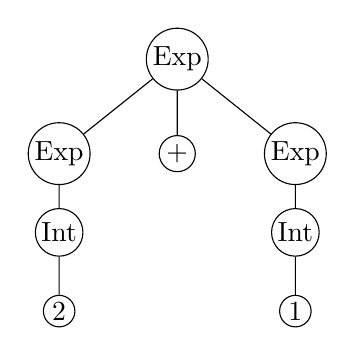
\begin{tikzpicture}[
  level 1/.style={sibling distance=15mm, level distance=12mm},
  level 2/.style={sibling distance=10mm, level distance=10mm},
  every node/.style={draw, circle, minimum size=4mm, inner sep=1pt}
]
  \node {Exp}
    child {node {Exp} 
      child {node {Int} 
        child {node {2}}}
    }
    child {node {+}}
    child {node {Exp}
      child {node {Int}
        child {node {1}}}
    };
\end{tikzpicture}
\end{minipage}
\hfill
\begin{minipage}{0.45\textwidth}
$1 + 2 * 3$ \\
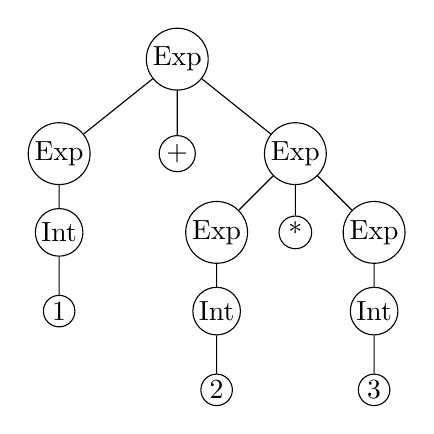
\begin{tikzpicture}[
  level 1/.style={sibling distance=15mm, level distance=12mm},
  level 2/.style={sibling distance=10mm, level distance=10mm},
  every node/.style={draw, circle, minimum size=4mm, inner sep=1pt}
]
  \node {Exp}
    child {node {Exp}
      child {node {Int}
        child {node {1}}}
    }
    child {node {+}}
    child {node {Exp}
      child {node {Exp}
        child {node {Int}
          child {node {2}}}
      }
      child {node {*}}
      child {node {Exp}
        child {node {Int}
          child {node {3}}}
      }
    };
\end{tikzpicture}
\end{minipage}

\vspace{10mm} % Add vertical space between rows

\noindent
\begin{minipage}{0.45\textwidth}
$1 + (2 * 3)$ \\
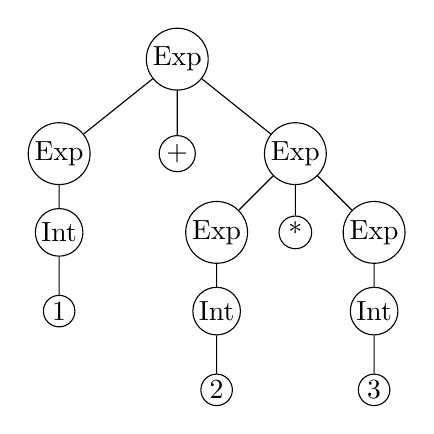
\begin{tikzpicture}[
  level 1/.style={sibling distance=15mm, level distance=12mm},
  level 2/.style={sibling distance=10mm, level distance=10mm},
  every node/.style={draw, circle, minimum size=4mm, inner sep=1pt}
]
  \node {Exp}
    child {node {Exp}
      child {node {Int}
        child {node {1}}}
    }
    child {node {+}}
    child {node {Exp}
      child {node {Exp}
        child {node {Int}
          child {node {2}}}
      }
      child {node {*}}
      child {node {Exp}
        child {node {Int}
          child {node {3}}}
      }
    };
\end{tikzpicture}
\end{minipage}
\hfill
\begin{minipage}{0.45\textwidth}
$(1 + 2) * 3$ \\
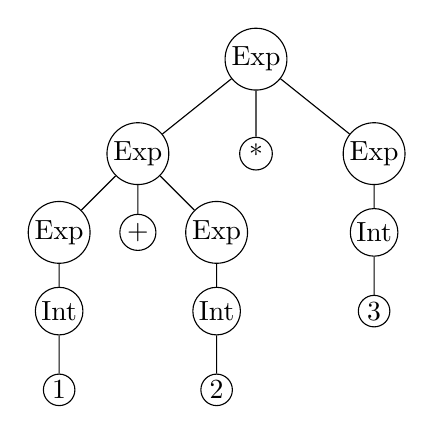
\begin{tikzpicture}[
  level 1/.style={sibling distance=15mm, level distance=12mm},
  level 2/.style={sibling distance=10mm, level distance=10mm},
  every node/.style={draw, circle, minimum size=4mm, inner sep=1pt}
]
  \node {Exp}
    child {node {Exp}
      child {node {Exp}
        child {node {Int}
          child {node {1}}}
      }
      child {node {+}}
      child {node {Exp}
        child {node {Int}
          child {node {2}}}
      }
    }
    child {node {*}}
    child {node {Exp}
      child {node {Int}
        child {node {3}}}
    };
\end{tikzpicture}
\end{minipage}

\vspace{10mm} % Add vertical space between rows

\noindent
\begin{minipage}{\textwidth}
$1 + 2 * 3 + 4 * 5 + 6$

\begin{center}
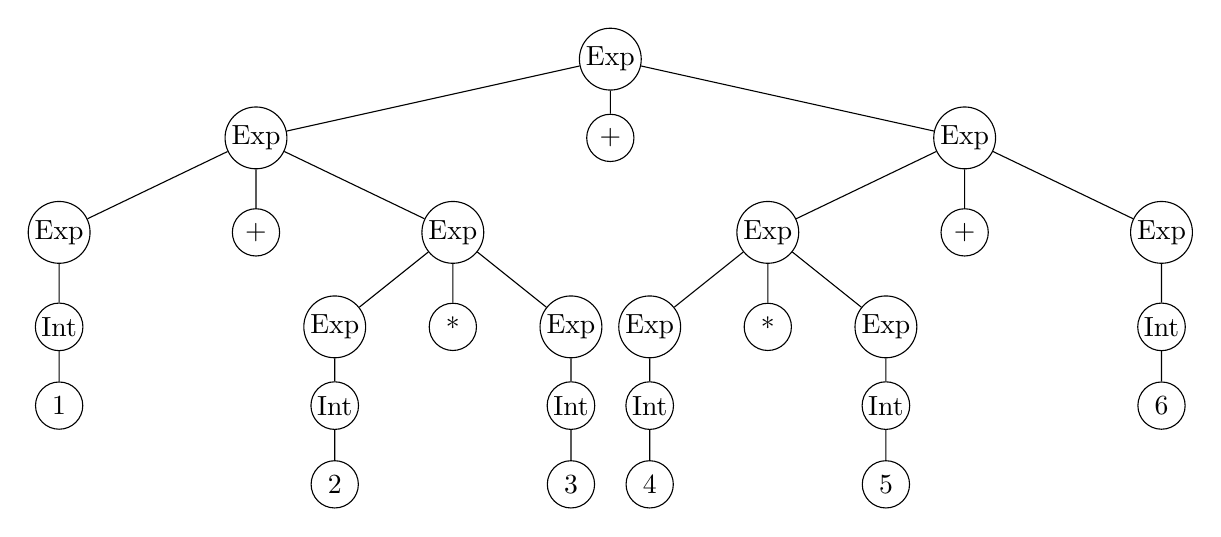
\begin{tikzpicture}[
  level 1/.style={sibling distance=45mm, level distance=10mm},
  level 2/.style={sibling distance=25mm, level distance=12mm},
  level 3/.style={sibling distance=15mm, level distance=12mm},
  level 4/.style={sibling distance=15mm, level distance=10mm},
  every node/.style={draw, circle, minimum size=6mm, inner sep=1pt}
]

  \node {Exp}
    child {node {Exp}
      child {node {Exp}
        child {node {Int} 
          child {node {1}}}
      }
      child {node {+}}
      child {node {Exp}
        child {node {Exp}
          child {node {Int}
            child {node {2}}}
        }
        child {node {*}}
        child {node {Exp}
          child {node {Int}
            child {node {3}}}
        }
      }
    }
    child {node {+}}
    child {node {Exp}
      child {node {Exp}
        child {node {Exp}
          child {node {Int}
            child {node {4}}}
        }
        child {node {*}}
        child {node {Exp}
          child {node {Int}
            child {node {5}}}
        }
      }
      child {node {+}}
      child {node {Exp}
        child {node {Int}
          child {node {6}}}
      }
    };

\end{tikzpicture}
\end{center}
\end{minipage}


\subsubsection*{Comments and Questions}

My question for this week is the following: How can this concept of parcing be applied to the developement of a programming language, specifically in the ways in which the backend handles order of operations regarding actual code as opposed to just calculations like we did in our calculators?

\subsection{Week 5}



\subsubsection*{Notes}
This week, we began discussing logical propositions and operations, starting with a real-world example: Proposition P ("It is raining") and Proposition Q ("The street is wet"). Using Lean, we explored how logical reasoning principles can provide proofs for statements like `n = 0 → n + 1 = 1`. We examined propositions as data types that can be true or false, with examples showing how conjunctions (P ∧ Q) require evidence, or "witnesses," to prove both components. Through diagrams and rules like formation, introduction, and elimination, we deepened our understanding of logical systems. The readings supported these concepts, introducing Gödel, Escher, Bach's explanation of propositional calculus and Lean's role as both a functional programming language and a proof assistant. They also explored propositional and predicate logic, covering syntax, connectives, inference rules, and the validation of logical arguments, emphasizing formal logic's foundational role in programming languages and mathematics.

\subsubsection*{Homework}

\medskip\noindent\centerline{\underline{Level 1}}
\begin{minted}{lean}
  variables P : Prop

  -- Assume that P is on a to-do list, and we need to prove P.
  example (todo_list : P) : P :=
  begin
    -- Directly use the given assumption to complete the proof.
    exact todo_list,
  end
\end{minted}

\medskip\noindent\centerline{\underline{Level 2}}

\begin{minted}{lean}
  variables P S : Prop
  example (p : P) (s : S) : P ∧ S :=
  begin
     -- Use the and.intro rule to construct the conjunction.
     exact and.intro p s,
   end
\end{minted}

\medskip\noindent\centerline{\underline{Level 3}}

\begin{minted}{lean}
  variables A I O U : Prop
  example (a : A) (i : I) (o : O) (u : U) : (A ∧ I) ∧ O ∧ U :=
  begin
    -- Combine the propositions step by step using nested and.intro.
    exact ⟨⟨a, i⟩, ⟨o, u⟩⟩,
  end
\end{minted}

\medskip\noindent\centerline{\underline{Level 4}}

\begin{minted}{lean}
  variables P S : Prop
  example (vm : P ∧ S) : P :=
  begin
    -- Use and.left to extract P from the conjunction.
    have p := and.left vm,
    -- Conclude the proof with the extracted value.
    exact p,
  end
\end{minted}

\medskip\noindent\centerline{\underline{Level 5}}

\begin{minted}{lean}
  variables P Q : Prop
  example (h : P ∧ Q) : Q :=
  begin
    -- Use and.right to extract Q from the conjunction.
    exact h.right,
  end
\end{minted}

\medskip\noindent\centerline{\underline{Level 6}}

\begin{minted}{lean}
  variables A I O U : Prop
  example (h1 : A ∧ I) (h2 : O ∧ U) : A ∧ U :=
  begin
    -- Extract A from h1.
    have a := h1.left,
    -- Extract U from h2.
    have u := h2.right,
    -- Combine A and U using and.intro.
    exact and.intro a u,
  end
\end{minted}

\medskip\noindent\centerline{\underline{Level 7}}

\begin{minted}{lean}
  variables C L : Prop
  example (h : (L ∧ ((L ∧ C) ∧ L) ∧ L ∧ L ∧ L) ∧ (L ∧ L) ∧ L) : C :=
  begin
    -- Extract the left-hand side of the conjunction.
    have h₁ := h.left,
    -- Navigate through the structure to isolate C.
    exact h.left.right.left.left.right,
  end
\end{minted}

\medskip\noindent\centerline{\underline{Level 8}}

\begin{minted}{lean}
  variables A C I O P S U : Prop
  example (h : ((P ∧ S) ∧ A) ∧ ¬I ∧ (C ∧ ¬O) ∧ ¬U) : A ∧ C ∧ P ∧ S :=
  begin
    -- Extract the conjunction (P ∧ S) ∧ A.
    have h₁ := h.left,
    -- Separate P ∧ S and A.
    have ps := h₁.left,
    have a := h₁.right,
    -- Extract (C ∧ ¬O) and isolate C.
    have h₂ := h.right.right.left,
    have c := h₂.left,
    -- Combine A, C, P, and S using and.intro.
    exact ⟨a, c, ps.left, ps.right⟩,
  end
\end{minted}

Mathematical Proof for Level 8:
\begin{align*}
  &= ((P \land S) \land A) \land \neg I \land (C \land \neg O) \land \neg U  & \text{assumption} \\
  &= (P \land S) \land A  & \text{and\_left (1)} \\
  &= P \land S  & \text{and\_left (2)} \\
  &= A  & \text{and\_right (2)} \\
  &= C \land \neg O  & \text{and\_right (1)} \\
  &= C  & \text{and\_left (5)} \\
  &= P  & \text{and\_left (3)} \\
  &= S  & \text{and\_right (3)} \\
  &= A \land C \land P \land S  & \text{and\_intro (4) (6) (7) (8)}
\end{align*}


\subsubsection*{Comments and Questions}

How can Lean logic proofs enhance our understanding of programming languages, particularly in verifying program correctness and exploring foundational concepts like recursion, type systems, and propositions?


\subsection{Week 6}

\subsubsection*{Notes}
This week, we explored lambda calculus, its syntax, and its foundational role in programming languages. Lambda calculus simplifies functions into three constructs: lambda abstraction (e.g., \(\lambda x.x + 1\)), evaluation (e.g., \((\lambda x.x + x)2 \leadsto 4\)), and variables, focusing on computation without named functions. We discussed abstraction principles, alpha equivalence, and De Bruijn indices, highlighting the importance of variable substitution and avoiding conflicts via capture-avoiding substitution. Computation in lambda calculus was also compared to programming, emphasizing its non-symmetric nature and the precedence rules for left-associative applications. 


\subsubsection*{Homework}

Levels 1-8 of the ``\(\rightarrow\) Tutorial: Party Snacks'' from the Lean Logic Game.

\medskip\noindent\centerline{\underline{Level 1}}

\begin{minted}{lean}
  -- Show that the cake will be delivered to the party.
  variables P C : Prop
  example (p : P) (bakery_service : P → C) : C :=
  begin
    -- Use the bakery service to derive C (the cake) from P.
    exact (bakery_service p),
  end
\end{minted}

\medskip\noindent\centerline{\underline{Level 2}}

\begin{minted}{lean}
  -- Prove that a proposition implies itself (identity property).
  variables C : Prop
  example : C → C :=
  begin
    -- Use the identity function to establish C → C.
    exact λ h : C ↦ h
  end
\end{minted}

\medskip\noindent\centerline{\underline{Level 3}}

\begin{minted}{lean}
  -- Demonstrate that conjunction (∧) is commutative.
  variables I S : Prop
  example : I ∧ S → S ∧ I :=
  begin
    -- Use and_intro to swap h.right (S) and h.left (I).
    exact λ h => and_intro (h.right) (h.left),
  end
\end{minted}

\medskip\noindent\centerline{\underline{Level 4}}

\begin{minted}{lean}
  -- Prove the transitivity of implication (→).
  variables C A S : Prop
  example (h1 : C → A) (h2 : A → S) : C → S :=
  begin
    -- Apply h1 to derive A, then use h2 to obtain S.
    exact λ h => h2 (h1 h)
  end
\end{minted}

\medskip\noindent\centerline{\underline{Level 5}}

\begin{minted}{lean}
  -- Prove the chain of reasoning to derive U.
  variables P Q R S T U : Prop
  example (p : P) (h1 : P → Q) (h2 : Q → R) (h3 : Q → T) (h4 : S → T) (h5 : T → U) : U :=
  begin
    -- Use h1 to derive Q from P, apply h3 to get T, and h5 to get U.
    exact h5 (h3 (h1 p)),
  end
\end{minted}

\medskip\noindent\centerline{\underline{Level 6}}

\begin{minted}{lean}
  -- Explore how conjunction interacts with implication.
  variables C D S : Prop
  example (h : C ∧ D → S) : C → D → S :=
  begin
    -- Assume C and D, then use h on the pair ⟨c, d⟩.
    exact λ c d => h ⟨c, d⟩
  end
\end{minted}

\medskip\noindent\centerline{\underline{Level 7}}

\begin{minted}{lean}
  -- Reverse the interaction between conjunction and implication.
  variables C D S : Prop
  example (h : C → D → S) : C ∧ D → S :=
  begin
    -- Assume ⟨c, d⟩ is C ∧ D, then use h with c and d.
    exact λ ⟨c, d⟩ => h c d
  end
\end{minted}

\medskip\noindent\centerline{\underline{Level 8}}

\begin{minted}{lean}
  -- Show that implication distributes over conjunction.
  variables C D S : Prop
  example (h : (S → C) ∧ (S → D)) : S → C ∧ D :=
  begin
    -- Assume S, then use h.left for C and h.right for D.
    exact λ s => ⟨h.left s, h.right s⟩,
  end
\end{minted}

\subsection*{Comments and Questions}

My question for this week is how can some of the concepts we learned with different types of proofs be applied to lamda calculus proofs. And how can these lamda calculus proofs then be used in the developement of a programming language?

\subsection{Week 7}

\subsubsection*{Notes}
This week, we explored key concepts in lambda calculus, focusing on currying, uncurrying, logic encoding, and Church numerals. Starting with the goal of transforming \( h : (A \land B) \to C \) into \( h' : A \to (B \to C) \), we demonstrated how to abstract over variables using lambda notation, such as \( h' := \lambda a. \lambda b. h(a, b) \). Similarly, we reversed the process by defining \( k' := \lambda p. k(p.left, p.right) \) for uncurrying. Examples like addition for natural numbers illustrated the correspondence between curried and uncurried forms.

Next, we introduced constructs for logic encoding, such as \( \text{true}, \text{false}, \) and \( \text{if-then-else} \). These were defined as \( \text{true} := \lambda x. \lambda y. x \), \( \text{false} := \lambda x. \lambda y. y \), and \( \text{if-then-else} := \lambda x. \lambda y. \lambda z. xyz \). Logical operations like \( \text{not}, \text{and}, \text{or} \) were expressed using these constructs. For instance, \( \text{not} := \lambda x. x \, \text{false} \, \text{true} \), \( \text{and} := \lambda x. \lambda y. x \, y \, \text{false} \), and \( \text{or} := \lambda x. \lambda y. x \, \text{true} \, y \).

We explored evaluation strategies: applicative order (evaluating inner expressions first) and normal order (reducing outermost expressions first). Normal order ensures termination if possible but may be slower. Finally, Church numerals were introduced to encode arithmetic, with definitions like \( 1 := \lambda f. \lambda x. fx \), \( 2 := \lambda f. \lambda x. f(fx) \), and \( 0 := \lambda f. \lambda x. x \). Arithmetic operations, such as addition, were built upon this framework.

The week concluded with exercises evaluating expressions like \( \text{and true false} \), using substitution and beta reduction to demonstrate the equivalence of these constructs and reinforce their logical consistency.


\subsubsection*{Homework}

\paragraph{1. Simplify the following lambda expression:}

\begin{minted}[escapeinside=||]{haskell}
((λm.λn. m n) (λf.λx. f (f x))) (λf.λx. f (f (f x)))
\end{minted}

The reduction proceeds in 7 steps using beta reduction:

\begin{minted}[escapeinside=||]{haskell}
((λm.λn. m n) (λf.λx. f (f x))) (λf.λx. f (f (f x)))
|\squigglyarrow| (λn. (λf.λx. f (f x)) n) (λf.λx. f (f (f x)))    -- Replace m with (λf.λx. f (f x))
|\squigglyarrow| (λn. (λf.λx. f (f x)) (λf.λx. f (f (f x))))      -- Replace n with (λf.λx. f (f (f x)))
|\squigglyarrow| (λf.λx. f (f (f x)))                            -- Apply (λf.λx. f (f x))
|\squigglyarrow| (λf.λx. f (f (f (f (f x)))))                    -- Result: Church numeral 9
\end{minted}

\paragraph{2. Describe the natural number function implemented by \((λm.λn. m n)\):} 

\leavevmode

This lambda function represents application. It takes two arguments: a "function" \texttt{m} and an "element" \texttt{n}, then applies \texttt{m} to \texttt{n} exactly once.


\subsection*{Comments and Questions}
How does the process of simplifying lambda terms using beta reduction help us understand the computational behavior of functional programming languages?

\subsection{Week 8 and 9}

\subsubsection*{Notes}
In these weeks, we explored advanced extensions of lambda calculus, building on earlier topics like boolean logic, conditional constructs, and arithmetic operations such as numerals, addition, and exponentiation. A key focus was the introduction of the `let` construct, which enables the use of local variable names and supports recursion. Recursion, the ability of a function to reference itself, relies on `let` for implementation in the absence of explicit function names. This highlights how `let` expressions facilitate recursive behavior in lambda calculus. We also worked on developing a lambda calculus interpreter. This taught me a lot about lambda calculus and how it is implemented in programming languages.

\subsubsection*{Homework}
Excercises 2-8:

2. Explain why a b c d reduces to (((a b) c) d) and why (a) reduces to a:

In lambda calc. expressions such as a b c d are evaluated as nested applications because the function application is inheretly left-associative. In tha case of (a), parenthesis in lambda calculus are used for grouping 2 or more variables so since a is just one variable the parenthesis can be dropped leaving us with just a.

3. How does capture avoiding substitution work? Investigate both by making relevant test cases and by looking at the source code. How is it implemented?

Capture-avoiding substitution prevents accidental overlaps of variable names when replacing variables in an expression by renaming certain variables to keep them distinct. This process ensures that each variable keeps its intended meaning, even if it needs a new name to avoid conflicts during substitution. It is implemented by checking each variable before the substitution occurs

4. Do you always get the expected result? Do all computations reduce to normal form?

I got the expected result sometimes. Not all computations reduce to normal form because some lambda expressions can cause infinite loops.

5. What is the smallest lambda expression you can find (minimal working example, MWE) that does not reduce to normal form?

The smallest expresion that does not reduce to normal form is (lambdax.x x) (lambdax.x x)

6. no question asked here

7. How does the interpreter evaluate ((lambdam.lambdan. m n) (lambdaf.lambdax. f (f x))) (lambdaf.lambdax. f (f (f x)))? Do a calculation similarly to when you evaluated ((lambdam.lambdan. m n) (lambdaf.lambdax. f (f x))) (lambdaf.lambdax. f (f (f x))) for the homework, but now follow precisely the steps taken by interpreter.py

Using the input:"((lambdam.lambdan. m n) (lambdaf.lambdax. f (f x))) (lambdaf.lambdax. f (f (f x)))"

Substitute called: replacing m with (lambdaf.(lambdax.(f (f x)))) in (lambdan.(m n))

Proceeding with substitution in lambda body for n

Substitute called: replacing m with (lambdaf.(lambdax.(f (f x)))) in (m n)

Substitute called: replacing m with (lambdaf.(lambdax.(f (f x)))) in m

Substituting variable m with (lambdaf.(lambdax.(f (f x))))

Substitute called: replacing m with (lambdaf.(lambdax.(f (f x)))) in n

Substitute called: replacing n with (lambdaf.(lambdax.(f (f (f x))))) in ((lambdaf.(lambdax.(f (f x)))) n)

Substitute called: replacing n with (lambdaf.(lambdax.(f (f (f x))))) in (lambdaf.(lambdax.(f (f x))))

Proceeding with substitution in lambda body for f

Substitute called: replacing n with (lambdaf.(lambdax.(f (f (f x))))) in (lambdax.(f (f x)))

Proceeding with substitution in lambda body for x

Substitute called: replacing n with (lambdaf.(lambdax.(f (f (f x))))) in (f (f x))

Substitute called: replacing n with (lambdaf.(lambdax.(f (f (f x))))) in f

Substitute called: replacing n with (lambdaf.(lambdax.(f (f (f x))))) in (f x)

Substitute called: replacing n with (lambdaf.(lambdax.(f (f (f x))))) in f

Substitute called: replacing n with (lambdaf.(lambdax.(f (f (f x))))) in x

Substitute called: replacing n with (lambdaf.(lambdax.(f (f (f x))))) in n

Substituting variable n with (lambdaf.(lambdax.(f (f (f x)))))

Substitute called: replacing f with (lambdaf.(lambdax.(f (f (f x))))) in (lambdax.(f (f x)))

Proceeding with substitution in lambda body for x

Substitute called: replacing f with (lambdaf.(lambdax.(f (f (f x))))) in (f (f x))

Substitute called: replacing f with (lambdaf.(lambdax.(f (f (f x))))) in f

Substituting variable f with (lambdaf.(lambdax.(f (f (f x)))))

Substitute called: replacing f with (lambdaf.(lambdax.(f (f (f x))))) in (f x)

Substitute called: replacing f with (lambdaf.(lambdax.(f (f (f x))))) in f

Substituting variable f with (lambdaf.(lambdax.(f (f (f x)))))

Substitute called: replacing f with (lambdaf.(lambdax.(f (f (f x))))) in x
(lambdax.((lambdaf.(lambdax.(f (f (f x))))) ((lambdaf.(lambdax.(f (f (f x))))) x)))

8. Write out the trace of the interpreter in the format we used to picture the recursive trace of hanoi. Only write lines that contain calls to evaluate() or calls tosubstitute()[4]. Add the line numbers

12: eval(('app', ('app', ('lam', 'm', ('lam', 'n', ('app', ('var', 'm'), ('var', 'n')))), ('lam', 'f', ('lam', 'x', ('app', ('var', 'f'), ('app', ('var', 'f'), ('var', 'x')))))), ('lam', 'f', ('lam', 'x', ('app', ('var', 'f'), ('app', ('var', 'f'), ('app', ('var', 'f'), ('var', 'x'))))))))

12: eval(('app', ('lam', 'm', ('lam', 'n', ('app', ('var', 'm'), ('var', 'n')))), ('lam', 'f', ('lam', 'x', ('app', ('var', 'f'), ('app', ('var', 'f'), ('var', 'x')))))))

12: eval(('lam', 'm', ('lam', 'n', ('app', ('var', 'm'), ('var', 'n')))))

51: Returning ('lam', 'm', ('lam', 'n', ('app', ('var', 'm'), ('var', 'n'))))

39: substitute(('lam', 'n', ('app', ('var', 'm'), ('var', 'n'))), m, ('lam', 'f', ('lam', 'x', ('app', ('var', 'f'), ('app', ('var', 'f'), ('var', 'x'))))))

60: substitute(('lam', 'n', ('app', ('var', 'm'), ('var', 'n'))), m, ('lam', 'f', ('lam', 'x', ('app', ('var', 'f'), ('app', ('var', 'f'), ('var', 'x'))))))

60: substitute(('app', ('var', 'm'), ('var', 'n')), m, ('lam', 'f', ('lam', 'x', ('app', ('var', 'f'), ('app', ('var', 'f'), ('var', 'x'))))))

60: substitute(('var', 'm'), m, ('lam', 'f', ('lam', 'x', ('app', ('var', 'f'), ('app', ('var', 'f'), ('var', 'x'))))))

64: Returning ('lam', 'f', ('lam', 'x', ('app', ('var', 'f'), ('app', ('var', 'f'), ('var', 'x')))))

60: substitute(('var', 'n'), m, ('lam', 'f', ('lam', 'x', ('app', ('var', 'f'), ('app', ('var', 'f'), ('var', 'x'))))))

64: Returning ('var', 'n')

\subsection*{Comments and Questions}
Week 8: How can we use lambda calculus to perform tasks in different orders when managing a tasks in a programming language?

Week 9: What implications does lambda calculus have on the functionality of programming languages? How is it implemented? Is there an easier and more efficient implementing capture-avoiding substitution in the interpreter?


\subsection{Week 10}

\subsubsection*{Notes}
This week, we explored rewriting theory, which transforms expressions into new forms and underpins computation in various fields. We discussed rewrite rules in systems like Turing machines and their application to processes such as the "MU game" and the Collatz sequence. Rewriting systems are formalized as \((A, R)\), where \(A\) is a set of terms and \(R\) defines transformations, often visualized as directed graphs. Key properties include confluence, ensuring all reduction paths lead to the same result, and termination, guaranteeing computations eventually stop. Normal forms, representing irreducible terms, play a crucial role in this framework. Practical examples, such as bubble sort, highlight rewriting's ability to formalize algorithms and ensure predictable outcomes in computation.


\subsubsection*{Homework}
Questions of Reflection from Assignment 3

1) What did you find most challenging when working through Homework 8/9 and Assignment 3?

The most challenging part was implementing capture-avoiding substitution in the interpreter, especially ensuring that variable renaming didn’t accidentally change the meaning of expressions. Tracking variable scopes and managing recursive evaluations required careful debugging and a solid understanding of lambda calculus mechanics, which was conceptually and technically demanding.

2) How did you come up with the key insight for Assignment 3?

The key insight came from breaking down each component of the interpreter into smaller, testable parts. By isolating the substitution mechanism and testing it with minimal expressions, I could see how substitutions worked in different cases. This modular approach helped me catch issues early on and better understand the flow of lambda expressions through the interpreter.

3) What is your most interesting takeaway from Homework 8/9 and Assignment 3?

The most interesting takeaway was realizing how lambda calculus can be used to simulate computation purely through function applications, without any inherent notion of numbers, operators, or other primitives. Building an interpreter from scratch gave me a deeper appreciation of how abstract computation principles can be directly implemented in code, connecting theory with practice in a very hands-on way

\subsection*{Comments and Questions}

How do the properties of confluence and termination in rewriting systems impact the reliability and predictability of algorithms, such as sorting algorithms or computational models like Turing machines? What is the application of interpreters like this in real-world systems?


\subsection{Week 11}

\subsubsection*{Notes}
This week, we discussed confluence and termination in abstract rewriting systems (ARS), defined as a pair \((A, R)\) where \(A\) is a set and \(R\) a binary relation. Confluence ensures that computations starting from the same element can always reach a common result, which is critical for guaranteeing consistency. Termination, or strict normalization, ensures no infinite computation paths exist, whereas weak normalization only guarantees that every element has a normal form, even if some paths are infinite. For example, a rewrite system with rules like \(aa \to a\) or \(ab \to b\) may always terminate, reducing to a single normal form. However, systems like \(a \to a\) and \(a \to b\) highlight that weak normalization does not imply termination, as infinite loops can occur. Conversely, terminating systems are always normalizing since all computations end in normal forms. These concepts underpin programming languages, aiding in understanding evaluation consistency and efficiency.


\subsubsection*{Homework}

\textbf{1.} \( A = \emptyset \)
\begin{center}
  This ARS represents an empty set
\end{center}
\hspace*{0.6cm}1. Yes ARS terminating. \\
\hspace*{0.6cm}2. Yes ARS confluent. \\
\hspace*{0.6cm}3. Yes has unique normal forms.

\textbf{2.} \( A = \{a\}, R = \emptyset \)
\begin{center}
  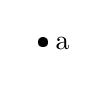
\begin{tikzpicture}
      \node (a) at (0,0) {\textbullet \,a};
  \end{tikzpicture}
\end{center}
\hspace*{0.6cm}1. Yes ARS terminating. \\
\hspace*{0.6cm}2. Yes ARS confluent. \\
\hspace*{0.6cm}3. Yes has unique normal forms.

\textbf{3.} \( A = \{a\}, R = \{(a, a)\} \)
\begin{center}
  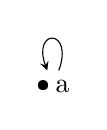
\begin{tikzpicture}[->, >=stealth]
      \node (a) at (0, 0) {\textbullet \,a};
      \draw [->] (a) to [out=70, in=110, looseness=10] (a);
  \end{tikzpicture}
\end{center}
\hspace*{0.6cm}1. No ARS not terminating. \\
\hspace*{0.6cm}2. Yes ARS confluent. \\
\hspace*{0.6cm}3. No does not have unique normal forms.

\textbf{4.} \( A = \{a, b, c\}, R = \{(a, b), (a, c)\} \)
\begin{center}
  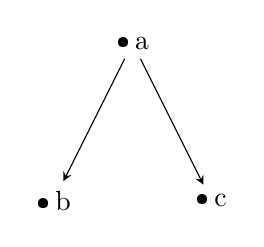
\begin{tikzpicture}[->, >=stealth]
      \node (a) at (0, 1) {\textbullet \,a};
      \node (b) at (-1, -1) {\textbullet \,b};
      \node (c) at (1, -1) {\textbullet \,c};
      \draw [->] (a) -- (b);
      \draw [->] (a) -- (c);
  \end{tikzpicture}
\end{center}
\hspace*{0.6cm}1. Yes ARS terminating. \\
\hspace*{0.6cm}2. No ARS not confluent. \\
\hspace*{0.6cm}3. No does not have unique normal forms.

\textbf{5.} \( A = \{a, b\}, R = \{(a, a), (a, b)\} \)
\begin{center}
  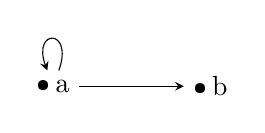
\begin{tikzpicture}[->, >=stealth]
      \node (a) at (0, 0) {\textbullet \,a};
      \node (b) at (2, 0) {\textbullet \,b};
      \draw [->] (a) to [out=70, in=110, looseness=10] (a);
      \draw [->] (a) -- (b);
  \end{tikzpicture}
\end{center}
\hspace*{0.6cm}1. No ARS not terminating. \\
\hspace*{0.6cm}2. Yes ARS confluent. \\
\hspace*{0.6cm}3. No does not have unique normal forms.

\textbf{6.} \( A = \{a, b, c\}, R = \{(a, b), (b, b), (a, c)\} \)
\begin{center}
  \begin{tikzpicture}[->, >=stealth]
      \node (a) at (0, 1.5) {\textbullet \,a};
      \node (b) at (2, 1.5) {\textbullet \,b};
      \node (c) at (1, 0) {\textbullet \,c};
      \draw [->] (a) -- (b);
      \draw [->] (b) to [out=70, in=110, looseness=10] (b);
      \draw [->] (a) -- (c);
  \end{tikzpicture}
\end{center}
\hspace*{0.6cm}1. No ARS not terminating. \\
\hspace*{0.6cm}2. Yes ARS confluent. \\
\hspace*{0.6cm}3. No does not have unique normal forms.

\textbf{7.} \( A = \{a, b, c\}, R = \{(a, b), (b, b), (a, c), (c, c)\} \)
\begin{center}
  \begin{tikzpicture}[->, >=stealth]
      \node (a) at (0, 1.5) {\textbullet \,a};
      \node (b) at (2, 1.5) {\textbullet \,b};
      \node (c) at (1, 0) {\textbullet \,c};
      \draw [->] (a) -- (b);
      \draw [->] (b) to [out=70, in=110, looseness=10] (b);
      \draw [->] (a) -- (c);
      \draw [->] (c) to [out=250, in=290, looseness=10] (c);
  \end{tikzpicture}
\end{center}
\hspace*{0.6cm}1. No ARS not terminating. \\
\hspace*{0.6cm}2. No ARS not confluent. \\
\hspace*{0.6cm}3. No does not have unique normal forms.
```

\subsection*{Comments and Questions}

How can ARS's improve the reliability and efficiency of modern programming languages in verifying complex code bases, especially in safety-critical applications like autonomous vehicles or financial systems? 


\subsection{Week 12}

\subsubsection*{Notes}
This week, we reviewed key concepts of Abstract Rewriting Systems (ARS). An ARS \((A, \to)\) consists of a set \(A\) (e.g., terms or expressions) and a binary relation \(\to\) that defines how elements can be rewritten. Key properties include termination (no infinite rewrite sequences), confluence (any two rewrite paths from the same starting point can join at a common successor), normalization (every element has at least one normal form), and unique normal forms (if normal forms exist, they are unique). Confluence does not guarantee normalization, but it ensures that any existing normal forms are unique. Examples of confluence include bubble sort, where the rule \(ba \to ab\) ensures a sorted, unique result (e.g., \(ab\)), lambda calculus, where beta reduction produces unique outcomes, and calculator arithmetic, which yields consistent results when following precedence rules. The Church-Rosser property extends confluence by ensuring that equivalent elements can join at a common successor. Confluence is critical in programming for deterministic outputs, and invariants, such as maintaining a consistent result during computation, help verify properties like termination and confluence.


\subsubsection*{Homework}

\subsection*{Exercise 1}
\textbf{Rewrite rule:} \( ba \to ab \)
\begin{enumerate}
    \item \textbf{Why does the ARS terminate?} The ARS terminates because each rewrite step decreases the number of inversions in the string, eventually reaching a sorted form.
    \item \textbf{What is the result of a computation (the normal form)?} The normal form is the string where all \( a \)'s precede all \( b \)'s.
    \item \textbf{Show that the result is unique (the ARS is confluent).} Confluence holds because any two paths lead to the same sorted result.
    \item \textbf{What specification does this algorithm implement?} The ARS implements a sorting algorithm that orders \( a \)'s before \( b \)'s.
\end{enumerate}

\subsection*{Exercise 2}
\textbf{Rewrite rules:} 
\[
\begin{aligned}
    aa &\to a, \\
    bb &\to a, \\
    ab &\to b, \\
    ba &\to b
\end{aligned}
\]
\begin{enumerate}
    \item \textbf{Why does the ARS terminate?} The ARS terminates because each rewrite step reduces the length of the string.
    \item \textbf{What are the normal forms?} The normal forms are either \( a \) or \( b \).
    \item \textbf{Is there a string \( s \) that reduces to both \( a \) and \( b \)?} No, the ARS is confluent, so each string reduces to a unique normal form.
    \item \textbf{Replacing \( \to \) with \( = \), which words become equal?} Any string with an even number of \( a \)'s and \( b \)'s reduces to \( a \), and strings with an odd number reduce to \( b \).
    \item \textbf{Which specification does the algorithm implement?} The ARS determines the parity of the total count of \( a \)'s and \( b \)'s, with \( a \) representing even and \( b \) representing odd.
\end{enumerate}

\subsection*{Exercise 3}
\textbf{Rewrite rules:} 
\[
\begin{aligned}
    aa &\to a, \\
    bb &\to b, \\
    ab &\to ba, \\
    ba &\to ab
\end{aligned}
\]
\begin{enumerate}
    \item \textbf{Why does the ARS not terminate?} The rules \( ab \to ba \) and \( ba \to ab \) create an infinite loop for certain strings.
    \item \textbf{What are the normal forms?} There are no normal forms due to the non-termination.
    \item \textbf{Modify the ARS to make it terminating with unique normal forms:} Add \( ab \to a \) or \( ba \to b \) to break the loop and ensure termination.
    \item \textbf{What specification does the ARS implement?} It simplifies strings by collapsing repeated letters and ordering \( a \)'s and \( b \)'s deterministically.
\end{enumerate}

\subsection*{Exercise 4}
\textbf{Rewrite rules:} 
\[
\begin{aligned}
    ab &\to ba, \\
    ba &\to ab
\end{aligned}
\]
\begin{enumerate}
    \item Same questions as Exercise 1. This ARS represents a basic sorting algorithm where the strings are reordered to have all \( a \)'s followed by all \( b \)'s.
\end{enumerate}

\subsection*{Exercise 5}
\textbf{Rewrite rules:} 
\[
\begin{aligned}
    ab &\to ba, \\
    ba &\to ab, \\
    aa &\to \varepsilon, \\
    b &\to \varepsilon
\end{aligned}
\]
\begin{enumerate}
    \item \textbf{Reduce some example strings such as \( abba \) and \( bababa \).}
        \begin{itemize}
            \item \( abba \to baba \to abab \to aabb \to \varepsilon \)
            \item \( bababa \to ababab \to aabbab \to aababb \to \varepsilon \)
        \end{itemize}
    \item \textbf{Why is the ARS not terminating?} The rules \( ab \to ba \) and \( ba \to ab \) create infinite loops.
    \item \textbf{How many equivalence classes does \( \leftrightarrow^\ast \) have? Can you describe them?} Two equivalence classes: strings reducing to \( \varepsilon \) and those that do not.
    \item \textbf{Can you change the rules to make the ARS terminating without changing equivalence classes?} Modify \( ab \to \varepsilon \) or \( ba \to \varepsilon \) to eliminate infinite loops.
    \item \textbf{Write questions about strings:} What is the shortest representation of a string? Does every string reduce to \( \varepsilon \)?
\end{enumerate}

\subsection*{Exercise 5b}
\textbf{Rewrite rules:}
\[
\begin{aligned}
    ab &\to ba, \\
    ba &\to ab, \\
    aa &\to a, \\
    b &\to \varepsilon
\end{aligned}
\]
\begin{enumerate}
    \item \textbf{Reduce some example strings such as \( abba \) and \( bababa \).}
        \begin{itemize}
            \item \( abba \to baba \to abab \to aabb \to ab \to ba \to a \)
            \item \( bababa \to ababab \to aabbab \to aabab \to abab \to aabb \to ab \to a \)
        \end{itemize}
        Under these rules, strings reduce to either \( a \) or \( \varepsilon \), depending on the counts of \( a \)'s and \( b \)'s.

    \item \textbf{Why is the ARS not terminating?} The rules \( ab \to ba \) and \( ba \to ab \) can cause infinite loops if not further constrained.

    \item \textbf{How many equivalence classes does \( \leftrightarrow^\ast \) have? Can you describe them?}
        \begin{itemize}
            \item There are two equivalence classes: strings that reduce to \( a \) and those that reduce to \( \varepsilon \).
            \item These equivalence classes are determined by the parity of \( b \)'s in the original string: even \( b \)'s reduce to \( a \), and odd \( b \)'s reduce to \( \varepsilon \).
        \end{itemize}

    \item \textbf{Can you change the rules to make the ARS terminating without changing equivalence classes?}
        \begin{itemize}
            \item Modify \( ab \to \varepsilon \) or \( ba \to \varepsilon \) to eliminate potential infinite loops caused by cyclic rewrites.
            \item For instance, adding a rule \( ab \to a \) would force the system to terminate while preserving the equivalence classes.
        \end{itemize}

    \item \textbf{Write questions about strings:}
        \begin{itemize}
            \item How many steps are required for a string to reach its normal form?
            \item Given a string, does it always reduce to \( a \) or \( \varepsilon \), and how can we predict the result?
        \end{itemize}
\end{enumerate}


\subsection*{Comments and Questions}

How does the concept of confluence in Abstract Rewriting Systems (ARS) ensure consistency in computational processes, and why is it critical for programming languages to maintain deterministic outputs? Provide examples, such as bubble sort or lambda calculus, to illustrate your points.

\subsection{Week 13}

\subsubsection*{Notes}
This week, we explored invariants through a chessboard activity, showing the original 8x8 board could be covered using 32 tiles, but the mutilated board (missing two blue tiles) could not, as it breaks the invariant requiring equal white and blue tiles in each step. The normal forms were either a fully covered board or two isolated uncovered tiles, demonstrating a terminating ARS. We then discussed defining functions using \texttt{let} and recursion. Simple definitions like \texttt{let succ = λn.n+1} work directly, but recursive definitions like factorials require \texttt{let rec}, which ensures proper self-referencing through fixed-point combinators. Key reductions include \texttt{(let x = e1 in e2) = (λx.e2)e1} and \texttt{(let rec f = e1 in e2) = (fix(λf.e2))e1}.

\subsubsection*{Homework}

\textbf{Initial expression:}
\[
\text{let rec fact = } \lambda n.\ \text{if } n = 0 \text{ then } 1 \text{ else } n \cdot \text{fact } (n-1) \text{ in fact 3}
\]

\begin{enumerate}
    \item \textbf{Step-by-step computation:}
    \begin{itemize}
        \item \textbf{Definition of \texttt{let rec}:}
        \[
        \text{let rec fact = } \lambda n.\ \text{if } n = 0 \text{ then } 1 \text{ else } n \cdot \text{fact } (n-1) \text{ in fact 3}
        \]
        becomes
        \[
        \text{let fact = (fix } (\lambda f.\ \lambda n.\ \text{if } n = 0 \text{ then } 1 \text{ else } n \cdot f (n-1)) \text{) in fact 3.}
        \]

        \item \textbf{Definition of \texttt{let}:}
        \[
        \text{let fact = (fix } (\lambda f.\ \lambda n.\ \text{if } n = 0 \text{ then } 1 \text{ else } n \cdot f (n-1)) \text{) in fact 3}
        \]
        becomes
        \[
        \big((\lambda \text{fact}.\ \text{fact } 3)\ (\text{fix } (\lambda f.\ \lambda n.\ \text{if } n = 0 \text{ then } 1 \text{ else } n \cdot f (n-1)))\big).
        \]

        \item \textbf{\(\beta\)-reduction (substitute \texttt{fix F}):}
        \[
        \big((\lambda \text{fact}.\ \text{fact } 3)\ (\text{fix } (\lambda f.\ \lambda n.\ \text{if } n = 0 \text{ then } 1 \text{ else } n \cdot f (n-1)))\big)
        \]
        reduces to
        \[
        \big((\text{fix } (\lambda f.\ \lambda n.\ \text{if } n = 0 \text{ then } 1 \text{ else } n \cdot f (n-1)))\ 3\big).
        \]

        \item \textbf{Definition of \texttt{fix}:}
        \[
        \big((\text{fix } (\lambda f.\ \lambda n.\ \text{if } n = 0 \text{ then } 1 \text{ else } n \cdot f (n-1)))\ 3\big)
        \]
        becomes
        \[
        \big((\lambda f.\ \lambda n.\ \text{if } n = 0 \text{ then } 1 \text{ else } n \cdot f (n-1))\ (\text{fix } (\lambda f.\ \lambda n.\ \text{if } n = 0 \text{ then } 1 \text{ else } n \cdot f (n-1)))\big)(3).
        \]

        \item \textbf{Substitute \(n = 3\):}
        \[
        (\lambda n.\ \text{if } n = 0 \text{ then } 1 \text{ else } n \cdot (\text{fix } (\lambda f.\ \lambda n.\ \text{if } n = 0 \text{ then } 1 \text{ else } n \cdot f (n-1)))(n-1))(3)
        \]
        reduces to
        \[
        \text{if } 3 = 0 \text{ then } 1 \text{ else } 3 \cdot (\text{fix } (\lambda f.\ \lambda n.\ \text{if } n = 0 \text{ then } 1 \text{ else } n \cdot f (n-1)))(2).
        \]

        \item \textbf{Definition of \texttt{if}:}
        \[
        \text{if } 3 = 0 \text{ then } 1 \text{ else } 3 \cdot (\text{fix } (\lambda f.\ \lambda n.\ \text{if } n = 0 \text{ then } 1 \text{ else } n \cdot f (n-1)))(2)
        \]
        evaluates to
        \[
        3 \cdot (\text{fix } (\lambda f.\ \lambda n.\ \text{if } n = 0 \text{ then } 1 \text{ else } n \cdot f (n-1)))(2).
        \]

        \item \textbf{Repeat substitution and evaluation for \(n = 2, 1, 0\):}
        The computation proceeds as follows:
        \[
        3 \cdot (2 \cdot (1 \cdot 1)) = 6.
        \]
    \end{itemize}

    \item \textbf{Final result:} The computation of \texttt{fact 3} yields:
    \[
    \boxed{6}
    \]
\end{enumerate}


\subsection*{Comments and Questions}

What are the trade-offs in terms of readability, efficiency, and debugging when using fixed-point combinators compared to traditional recursive function definitions?

\section{Lessons from the Assignments}


\section{Conclusion}\label{conclusion}


\begin{thebibliography}{99}
\bibitem[BLA]{bla} Author, \href{https://en.wikipedia.org/wiki/LaTeX}{Title}, Publisher, Year.
\end{thebibliography}

\end{document}
